\documentclass[12pt]{article}

\usepackage[utf8]{inputenc}
\usepackage{datetime}
\usepackage{amsthm}
\usepackage{amsmath}
\usepackage{amssymb}
\usepackage{enumitem}
\usepackage[american]{babel}
\usepackage{matlab-prettifier}
\usepackage{graphicx}
\usepackage[makeroom]{cancel}
\usepackage{afterpage}
\usepackage{capt-of}
\usepackage{bm}

\DeclareMathOperator*{\argmin}{arg\,min}

\newcommand\independent{\protect\mathpalette{\protect\independenT}{\perp}}
\def\independenT#1#2{\mathrel{\rlap{$#1#2$}\mkern2mu{#1#2}}}

\newtheoremstyle{colon}{\topsep}{\topsep}{}{}{\bfseries}{:}{ }{}
\theoremstyle{colon}
\newtheorem{exercise}{Exercise}
\newtheorem*{answer}{Answer}

\title{ELE 538: Large-Scale Optimization \\ Homework 2}
\author{Zachary Hervieux-Moore}

\newdate{date}{26}{3}{2018}
\date{\displaydate{date}}

\begin{document}

\maketitle

\clearpage

\begin{exercise}
	\textbf{Conjugate subgradient theorem:} Suppose $f$ is convex. Show that the following two statements are equivalent.
	\begin{enumerate}[label=\roman*)]
		\item $\langle \bm{x}, \bm{y} \rangle = f(\bm{x}) + f^* (\bm{y})$
		\item $\bm{y} \in \partial f(\bm{x})$
	\end{enumerate}
	\textbf{Remark:} this also means that the above statements are equivalent to $\bm{x} \in \partial f^* (\bm{y})$.
\end{exercise}

\begin{answer}

	Starting from i),

	\begin{align*}
		\langle \bm{x}, \bm{y} \rangle &= f(\bm{x}) + f^*(\bm{y}) \\
		&= f(\bm{x}) + \sup_z \{ \langle \bm{z}, \bm{y} \rangle - f(\bm{z}) \}
	\end{align*}
	\begin{align*}
		&\Longleftrightarrow \langle \bm{x}, \bm{y} \rangle \geq f(\bm{x}) + \langle \bm{z}, \bm{y} \rangle - f(\bm{z}) \quad \forall \bm{z} \\
		&\Longleftrightarrow f(\bm{z}) \geq f(\bm{x}) + \langle \bm{z} - \bm{x}, \bm{y} \rangle \quad \forall \bm{z} \\
		&\Longleftrightarrow \bm{y} \in \partial f(\bm{x})
	\end{align*}

\end{answer}

\clearpage

\begin{exercise}
	\textbf{Alternating projections for LP feasibility:} We consider the problem of finding a point $\bm{x} \in \mathbb{R}^n$ that satisfies $\bm{A} \bm{x} = \bm{b}$, $\bm{x} \succeq 0$, where $\bm{A} \in \mathbb{R}^{m \times n}$, with $m < n$.

	\begin{enumerate}[label=\alph*)]
		\item Work out alternating projections for this problem. (In other words, explain how to compute (Euclidean) projections onto $\{\bm{x} | \bm{A} \bm{x} = \bm{b} \}$ and $\mathbb{R}_+^n$.)
		\item Implement your method, and try it on one or more problem instances with $m = 500$, $n = 2000$. With $\bm{x}^k$ denoting the $k^{th}$ iterate after projection onto $\mathbb{R}_+^n$, plot $\lVert \bm{A} \bm{x}^k - \bm{b} \rVert_2$, the residual of the equality constraint. (This should converge to zero; you can terminate when this norm is smaller than $10^{-5}$.)
		\item A general method that can speed up alternating projections is to over-project, which means replacing the simple projection $\bm{x}^+ = \mathcal{P}(\bm{x})$ with $\bm{x}^+ = \bm{x} + \gamma(\mathcal{P}(\bm{x}) - \bm{x})$, where $\gamma \in [1,2)$. (When $\gamma = 1$, this reduces to standard projection.) It is not hard to show that alternating projections, with over-projection, converges to a point in the intersection of the sets. Implement over-projection and experiment with the over-projection factor $\gamma$, observing the effect on the number of iterations required for convergence.
	\end{enumerate}

\end{exercise}

\begin{answer}
	\

	\begin{enumerate}[label=\alph*)]
		\item The projection onto $\{\bm{x} | \bm{A} \bm{x} = \bm{b} \}$ from a point $\bm{z}$ is solved by the following minimization problem
			\begin{gather*}
				\min_{\bm{x}} \frac{1}{2} \lVert \bm{x} - \bm{z} \rVert^2 \\
				\text{s.t. } \bm{A} \bm{x} = \bm{b} 
			\end{gather*}
			This is a convex problem and so it is well behaved so we just find the KKT conditions
			\begin{gather*}
				\bm{x} - \bm{z} + \bm{A}^T \lambda = 0 \\
				\bm{A} \bm{x} = \bm{b}
			\end{gather*}
			Manipulating the first equation
			\begin{gather*}
				\bm{A} \bm{x} - \bm{A} \bm{z} + \bm{A} \bm{A}^T \lambda = 0 \\
				\implies \lambda = (\bm{A} \bm{A}^T)^{-1} (\bm{A} \bm{z} - \bm{b})
			\end{gather*}
			Which gives us the solution
			\begin{gather*}
				\bm{x} = \bm{z} + \bm{A}^T (\bm{A} \bm{A}^T)^{-1} (\bm{b} - \bm{A} \bm{z})
			\end{gather*}
			Then, projecting onto $\mathbb{R}_+^n$ is simply making the negative entries equal to 0
			\begin{gather*}
				\mathcal{P}_{\mathbb{R}_+^n} (\bm{x})_i = \max(0, x_i) \quad \forall i
			\end{gather*}

		\item The code used to generate the figure is attached below. Figure 1 shows the convergence to a stationary point. However, due to round off errors with the large dimension size, Matlab does not converge to 0. It does for smaller problems ($m = 5, n = 2000$).

			\begin{center}
		        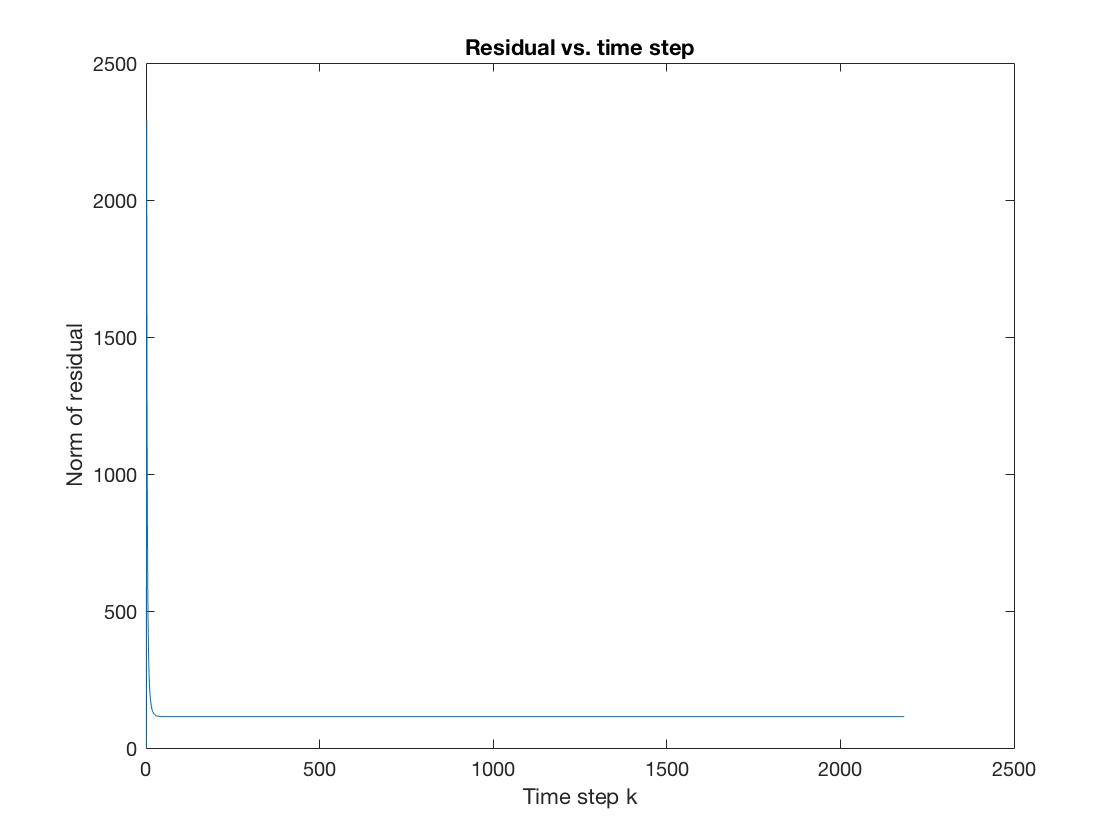
\includegraphics[width=0.8\textwidth]{2b.jpg}
		        \captionof{figure}{Plot of $\lVert \bm{A} \bm{x}^k - \bm{b} \rVert$}
			\end{center}

			\textbf{Code Appendix:}

			\begin{lstlisting}[style=Matlab-editor, basicstyle=\scriptsize]
clear;
clc;

m = 500;
n = 2000;

A = rand(m,n);
b = rand(m,1);
x(:,1) = rand(n,1);
i = 1;

while (norm(A*x(:,i) - b,2) > 10^-5)
    i = i + 1;
    % project into affine set
    x(:,i) = x(:,i-1) + A'/(A*A')*(b-A*x(:,i-1));
    
    i = i + 1;
    % project into positive orthant
    x(:,i) = max(0, x(:,i-1));
    
    res(ceil(i/2)) = norm(A*x(:,i) - b,2);
end

plot(res)
			\end{lstlisting}

		\item The code used to generate the figure is attached below. Notice that I used a smaller setting so that I got convergence so I could compare different $\lambda$. The figure below shows that convergence does speed up with an increased $\lambda$ but starts to slow down as $\lambda$ approaches 2.

			\begin{center}
		        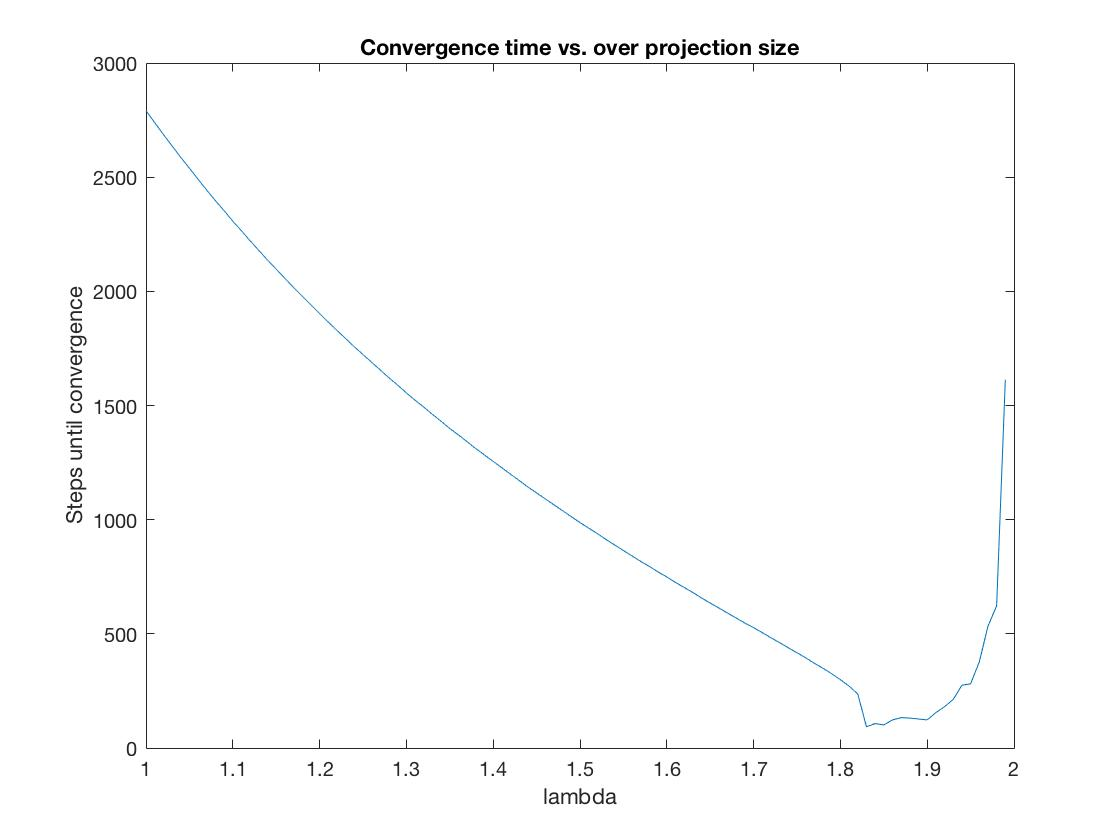
\includegraphics[width=0.8\textwidth]{2c.jpg}
		        \captionof{figure}{Plot of convergence time vs. $\lambda$}
			\end{center}

			\textbf{Code Appendix:}

			\begin{lstlisting}[style=Matlab-editor, basicstyle=\scriptsize]
clear;
clc;

m = 5;
n = 2000;

A = rand(m,n);
b = rand(m,1);
x(:,1) = zeros(n,1);
lambda = zeros(1,100);
j = 1;

for gamma=1:0.01:1.99
    clear x;
    x(:,1) = zeros(n,1);
    i = 1;
    while (norm(A*x(:,i) - b,2) > 10^-5)
        i = i + 1;
        % project into affine set
        x(:,i) = x(:,i-1) + gamma*(x(:,i-1) + A'/(A*A')*(b-A*x(:,i-1))-x(:,i-1));

        i = i + 1;
        % project into positive orthant
        x(:,i) = x(:,i-1) + gamma*(max(0, x(:,i-1))-x(:,i-1));
    end
    lambda(j) = i;
    j = j + 1;
end

plot(1:0.01:1.99, lambda)
			\end{lstlisting}
	\end{enumerate}

\end{answer}

\clearpage

\begin{exercise}
	\textbf{Minimizing expected Bregman divergence:} Let $\bm{z}$ be a random vector with distribution $\mathbb{P}$, and consider the following optimization problem
	\begin{gather*}
		\text{minimize}_{\bm{x}} \ \mathbb{E}_{\bm{z} \sim \mathbb{P}} [ D_{\varphi} (\bm{z}, \bm{x}) ]
	\end{gather*}
	for some strongly convex $\varphi$. Find the minimizer of this problem.
\end{exercise}

\begin{answer}
	We substitute the definition of Bregman divergence into the optimizaiton problem and check the first order conditions for an optimal point.
	\begin{align*}
		&\quad \ \text{minimize}_{\bm{x}} \ \mathbb{E}_{\bm{z} \sim \mathbb{P}} [ D_{\varphi} (\bm{z}, \bm{x}) ] \\
		&= \text{minimize}_{\bm{x}} \ \mathbb{E}_{\bm{z} \sim \mathbb{P}} [ \varphi(\bm{z}) - \varphi(\bm{x}) - \langle \nabla \varphi(\bm{x}), \bm{z} - \bm{x} \rangle] \\
		&= \text{minimize}_{\bm{x}} \ \langle \nabla \varphi(\bm{x}), \bm{x} - \mathbb{E}_{\bm{z} \sim \mathbb{P}} [\bm{z} ] \rangle - \varphi(\bm{x}) + \mathbb{E}_{\bm{z} \sim \mathbb{P}} [ \varphi(\bm{z})]
	\end{align*}
	Where we used the linearity of expectation to bring it into the inner product. Now, we take the gradient of the above with respect to $\bm{x}$.
	\begin{align*}
		\nabla_{\bm{x}} &\implies \nabla \varphi(\bm{x}) + \langle \nabla^2 \varphi(\bm{x}), \bm{x} - \mathbb{E}_{\bm{z} \sim \mathbb{P}} [\bm{z} ] \rangle - \nabla \varphi(\bm{x}) \\
		&= \langle \nabla^2 \varphi(\bm{x}), \bm{x} - \mathbb{E}_{\bm{z} \sim \mathbb{P}} [\bm{z} ] \rangle
	\end{align*}
	Of course, the above is equal to 0 if $\bm{x} = \mathbb{E}_{\bm{z} \sim \mathbb{P}} [\bm{z} ]$. Now, we must show that this is indeed a minimum. We need to check the second order conditions. So we differentiate with respect to $\bm{x}$ again and evaluate at $\bm{x} = \mathbb{E}_{\bm{z} \sim \mathbb{P}} [\bm{z} ]$.
	\begin{gather*}
		\nabla_{\bm{x}} \implies \langle \nabla^3 \varphi(\bm{x}), \bm{x} - \mathbb{E}_{\bm{z} \sim \mathbb{P}} [\bm{z} ] \rangle + \nabla^2 \varphi(\bm{x}) \\
		\bm{x} = \mathbb{E}_{\bm{z} \sim \mathbb{P}} [\bm{z} ] \implies \nabla^2 \varphi(\bm{x})
	\end{gather*}
	As $\varphi(\cdot)$ is strongly convex, we have that this is PSD and hence $\bm{x} = \mathbb{E}_{\bm{z} \sim \mathbb{P}} [\bm{z} ]$ is indeed a minimum.
\end{answer}

\clearpage

\begin{exercise}

	\textbf{Exponentiated gradient:}

	\begin{enumerate}[label=\alph*)]
		\item Consider the mirror descent update rule with KL divergence
			\begin{gather*}
				\bm{x}^{t+1} = \argmin_{\bm{x} \in \mathcal{C}} \left\{ f(\bm{x}^t) + \langle \nabla f(\bm{x}^t), \bm{x} - \bm{x}^t \rangle + \frac{1}{\eta_t} \text{KL}(\bm{x} \lVert \bm{x}^t) \right\}
			\end{gather*}
			where $KL(\bm{x} \lVert \bm{z}) := \sum_i x_i \log \frac{x_i}{z_i}$ and $\mathcal{C} = \Delta := \{ \bm{x} \in \mathbb{R}_+^n | \sum_{i=1}^n x_i = 1\}$. Show that if $\bm{x}^t \in \Delta$, then
			\begin{gather*}
				x_i^{t+1} = \frac{x_i^t \ \text{exp}(-\eta_t [\nabla f(\bm{x}^t)]_i)}{\sum_{j=1}^n x_j^t \ \text{exp}(-\eta_t [\nabla f(\bm{x}^t)]_j)}, \quad 1 \leq i \leq n
			\end{gather*}

		\item Consider the mirror descent update rule
			\begin{gather*}
				\bm{x}^{t+1} = \argmin_{\bm{x} \in \mathcal{C}} \left\{ f(\bm{x}^t) + \langle \nabla f(\bm{x}^t), \bm{x} - \bm{x}^t \rangle + \frac{1}{\eta_t} D_\varphi(\bm{x}, \bm{x}^t) \right\} 
			\end{gather*}
			where $D_\varphi(\bm{x}, \bm{z}) := \sum_i x_i \log \frac{x_i}{z_i} - x_i + z_i$ is the generalized KL divergence and $\mathcal{C} = \mathbb{R}_+^n$ is the positive orthant. When $\bm{x}^t \in \mathcal{C}$, find a closed-form expression for the mirror descent update.
	\end{enumerate}

\end{exercise}

\begin{answer}
	\

	\begin{enumerate}[label=\alph*)]
		\item As the function is differentiable, we simply differentiate and set to 0.
			\begin{align*}
				[\nabla_{\bm{x}}]_i &= [\nabla f(\bm{x}^t)]_i + \frac{1}{\eta_t} \left( \log \frac{x_i}{x_i^t} + 1 \right) = 0 \\
				&\implies \log \frac{x_i}{x_i^t} + 1 = -\eta_t [\nabla f(\bm{x}^t)]_i \\
				&\implies x_i = \frac{x_i^t \ \text{exp}(-\eta_t [\nabla f(\bm{x}^t)]_i)}{e}
			\end{align*}
			It is simple to check that this is indeed a minimum by checking the second order condition. Since $\bm{x}^t \in \Delta$, we have that all the components above are positive. However, we must normalize so that $\bm{x} \in \Delta$. Normalize by the $\lVert \cdot \rVert_1$ norm is justified as we are projecting onto $\Delta$. Thus,
			\begin{gather*}
				x_i^{t+1} = \frac{x_i}{\lVert \bm{x} \rVert_1} = \frac{x_i^t \ \text{exp}(-\eta_t [\nabla f(\bm{x}^t)]_i)}{\sum_{j=1}^n \bm{x}_j^t \ \text{exp}(-\eta_t [\nabla f(\bm{x}^t)]_j)} 
			\end{gather*}

		\item We repeat the procedure above
			\begin{align*}
				[\nabla_{\bm{x}}]_i &= [\nabla f(\bm{x}^t)]_i + \frac{1}{\eta_t} \left( \log \frac{x_i}{x_i^t} + 1 - 1 \right) = 0 \\
				&\implies x_i = x_i^t \ \text{exp}(-\eta_t [\nabla f(\bm{x}^t)]_i)
			\end{align*}
			Thus, we have $x_i^{t_1} = x_i^t \ \text{exp}(-\eta_t [\nabla f(\bm{x}^t)]_i)$ which is in the positive orthant as $x_i^t$ is aswell.

	\end{enumerate}

\end{answer}

\clearpage

\begin{exercise}

	\textbf{Proximal operators:}

	\begin{enumerate}[label=\alph*)]
		\item Suppose $f(\bm{x}) = \sum_{i=1}^n w_i \lvert x_i \rvert$ with $w_i \geq 0$. Computer $\text{prox}_f(\bm{x})$.

		\item Show that if $f(\bm{x}) = g(a \bm{x} + \bm{b})$ with $a \neq 0$, then
			\begin{gather*}
				\text{prox}_f(\bm{x}) = \frac{1}{a} ( \text{prox}_{a^2 g} (a \bm{x} + \bm{b}) - \bm{b})
			\end{gather*}

		\item Show that if $f(\bm{x}) = g(\bm{Q} \bm{x})$ with $\bm{Q}$ orthogonal (i.e. $\bm{Q} \bm{Q}^T = \bm{Q}^T \bm{Q} = \bm{I}$), then
			\begin{gather*}
				\text{prox}_f(\bm{x}) = \bm{Q}^T \text{prox}_g (\bm{Q} \bm{x})
			\end{gather*}

		\item Let $f(\bm{x}) = x_{[1]} + \cdots + x_{[k]}$, where $x_{[i]}$ is the $i^{th}$ largest entry of $\bm{x}$. Compute $\text{prox}_f (\bm{x})$.
	\end{enumerate}

\end{exercise}

\begin{answer}
	\

	\begin{enumerate}[label=\alph*)]
		\item We have
			\begin{gather*}
				\text{prox}_f(\bm{x}) = \argmin_{\bm{z}} \left\{ \frac{1}{2} \lVert \bm{z} - \bm{x} \rVert^2 + \sum_{i=1}^n w_i \lvert z_i \rvert \right\}
			\end{gather*}
			First, we handle the differentiable components. Again, we check first order and second order conditions. One yields
			\begin{gather*}
				z_i = x_i - w_i \text{ if } x_i > w_i \\
				z_i = x_i + w_i \text{ if } x_i < - w_i
			\end{gather*}
			Finally, between $-w_i \leq x_i \leq w_i$, we have that the quadratic term is smaller than the absolute term, so we pick $z_i = 0$ which defines the proximal operator for the 3 different cases.

		\item We have
			\begin{gather*}
				\text{prox}_f(\bm{x}) = \argmin_{\bm{z}} \left\{ \frac{1}{2} \lVert \bm{z} - \bm{x} \rVert^2 + g(a \bm{z} + b) \right\}
			\end{gather*}
			Manipulating the above, multiplying by a positive scalar ($a^2$) keeps the $\argmin$ unchanged,
			\begin{gather*}
				= \argmin_{\bm{z}} \left\{ \frac{1}{2} \lVert a \bm{z} + \bm{b} - a\bm{x} - \bm{b} \rVert^2 + a^2 g(a \bm{z} + \bm{b}) \right\} \\
				= \argmin_{\bm{z}'} \left\{ \frac{1}{2} \lVert \bm{z}' - a\bm{x} - \bm{b} \rVert^2 + a^2 g(\bm{z}') \right\}
			\end{gather*}
			Where we made the substitute $a \bm{z} + \bm{b} = \bm{z}'$. This is valid since the $\argmin$ is still over all $z' \in \mathbb{R}^n$. Thus, we have that $a \bm{z}^* + \bm{b} = \bm{z}'^*$ or $\text{prox}_f(\bm{x}) = \frac{1}{a} ( \text{prox}_{a^2 g} (a \bm{x} + \bm{b}) - \bm{b})$.

		\item We have
			\begin{gather*}
				\text{prox}_f(\bm{x}) = \argmin_{\bm{z}} \left\{ \frac{1}{2} \lVert \bm{z} - \bm{x} \rVert^2 + g(\bm{Q} \bm{z}) \right\} \\
				= \argmin_{\bm{z}} \left\{ \frac{1}{2} \lVert \bm{Q}^T \bm{Q} \bm{z} - \bm{Q}^T \bm{Q} \bm{x} \rVert^2 + g(\bm{Q} \bm{z}) \right\} \\
				= \argmin_{\bm{z}'} \left\{ \frac{1}{2} \lVert \bm{Q}^T \bm{z}' - \bm{Q}^T \bm{Q} \bm{x} \rVert^2 + g(\bm{z}') \right\}
			\end{gather*}
			Where the substitution $\bm{z}' = \bm{Q} \bm{z}$ is justified as $\bm{z}'$ still spans $\mathbb{R}^n$ by the orthogonality of $\bm{Q}$. Now, we also note by the orthogonality of $\bm{Q}$ that
			\begin{gather*}
				\lVert \bm{Q}^T \bm{z}' - \bm{Q}^T \bm{Q} \bm{x} \rVert^2 = \lVert \bm{z}' - \bm{Q} \bm{x} \rVert^2
			\end{gather*}
			Thus we have
			\begin{gather*}
				= \argmin_{\bm{z}'} \left\{\lVert \bm{z}' - \bm{Q} \bm{x} \rVert^2 + g(\bm{z}') \right\}
			\end{gather*}
			That is, $\bm{z}'^* = \bm{Q} \bm{z}^*$, or $\text{prox}_f(\bm{x}) = \bm{Q}^T \text{prox}_g (\bm{Q} \bm{x})$, as $\bm{Q}^{-1} = \bm{Q}^T$.

		\item We can rewrite $f(\bm{x})$ as $f(\bm{x}) = \sup_{\bm{y} \in \mathcal{C}} \bm{y}^T \bm{x}$ where $\mathcal{C} = \{ \bm{y} : 0 \preceq \bm{y} \preceq 1, 1^T \bm{y} = k \}$. That is, the solution to this optimization function is the $k$ largest entries of $\bm{x}$. Now we note that
			\begin{gather*}
				f^*(\bm{x}) = \delta_{\mathcal{C}}(\bm{x})
			\end{gather*}
			That is, the Fenchel conjugate of $f(\cdot)$ is the indicator function of $\mathcal{C}$. Now using Moreau decomposition, we have
			\begin{align*}
				\text{prox}_{f} (\bm{x}) &= \bm{x} - \text{prox}_{f^*} (\bm{x}) \\
				&= \bm{x} - \argmin_z \left\{ \frac{1}{2} \lVert \bm{z} - \bm{x} \rVert^2 + \delta_{\mathcal{C}} (\bm{z}) \right\} \\
				&= \bm{x} - \mathcal{P}_{\mathcal{C}}(\bm{x})
			\end{align*}
			That is, all one needs to do is compute the projection of $\bm{x}$ onto $\mathcal{C}$. Which is a projection onto a polyhedral set which is similar (different form) as to what was done in problem 2. The exact solution is easily derived using Lagrange multipliers.
	\end{enumerate}

\end{answer}

\clearpage

\begin{exercise}
	\textbf{Extended Moreau decomposition:} Let $f$ be closed and convex. Show that for any $\lambda > 0 $ and any $\bm{x}$, one has
	\begin{gather*}
		\bm{x} = \text{prox}_{\lambda f} (\bm{x}) + \lambda \text{prox}_{\frac{1}{\lambda} f^*} (\bm{x}/\lambda)
	\end{gather*}
\end{exercise}

\begin{answer}
	We prove this by applying Moreau decomposition to $\lambda f$. Recall that Moreau decomposition is
	\begin{gather*}
		\bm{x} = \text{prox}_{f} (\bm{x}) + \text{prox}_{f^*} (\bm{x})
	\end{gather*}
	So, we have to compute the conjugate of $\lambda f$ to get the Extended Moreau decomposition. So we have
	\begin{gather*}
		(\lambda f)^* (\bm{x}) = \sup_{\bm{z}} \left\{ \langle \bm{z}, \bm{x} \rangle - (\lambda f)(\bm{z}) \right\} 
	\end{gather*}
	Multiplying and dividing by $\lambda$ yields, we get that the above is equivalent to
	\begin{align*}
		&= \lambda \sup_{\bm{z}} \left\{ \langle \bm{z}, \bm{x}/\lambda \rangle - (f)(\bm{z}) \right\} \\
		&= \lambda f^*(\bm{x}/\lambda)
	\end{align*}
	Thus we have that $(\lambda f)^* (\bm{x}) = \lambda f^*(\bm{x}/\lambda)$ which we now plug into our proximal operator and use the fact proved in 5b) ($g = f^*, a = 1/\lambda, \bm{b}=0$) to get
	\begin{align*}
		\text{prox}_{(\lambda f)^*} (\bm{x}) &= \text{prox}_{\lambda g} (\bm{x}) \\
		&= \lambda \text{prox}_{\frac{1}{\lambda^2} \cdot \lambda g} (\bm{x} / \lambda) \\
		&= \lambda \text{prox}_{\frac{1}{\lambda} f^*} (\bm{x}/\lambda)
	\end{align*}
	Which proves the claim that
	\begin{gather*}
		\bm{x} = \text{prox}_{\lambda f} (\bm{x}) + \lambda \text{prox}_{\frac{1}{\lambda} f^*} (\bm{x}/\lambda)
	\end{gather*}
\end{answer}

\end{document}